\chapter*{Context Action Outcome}

All examples can be thought of as being made up of three parts: \emph{context}, \emph{action}, and \emph{outcome}.

In your groups, come up with definitions for these terms and write them in the shapes below:

\begin{center}
    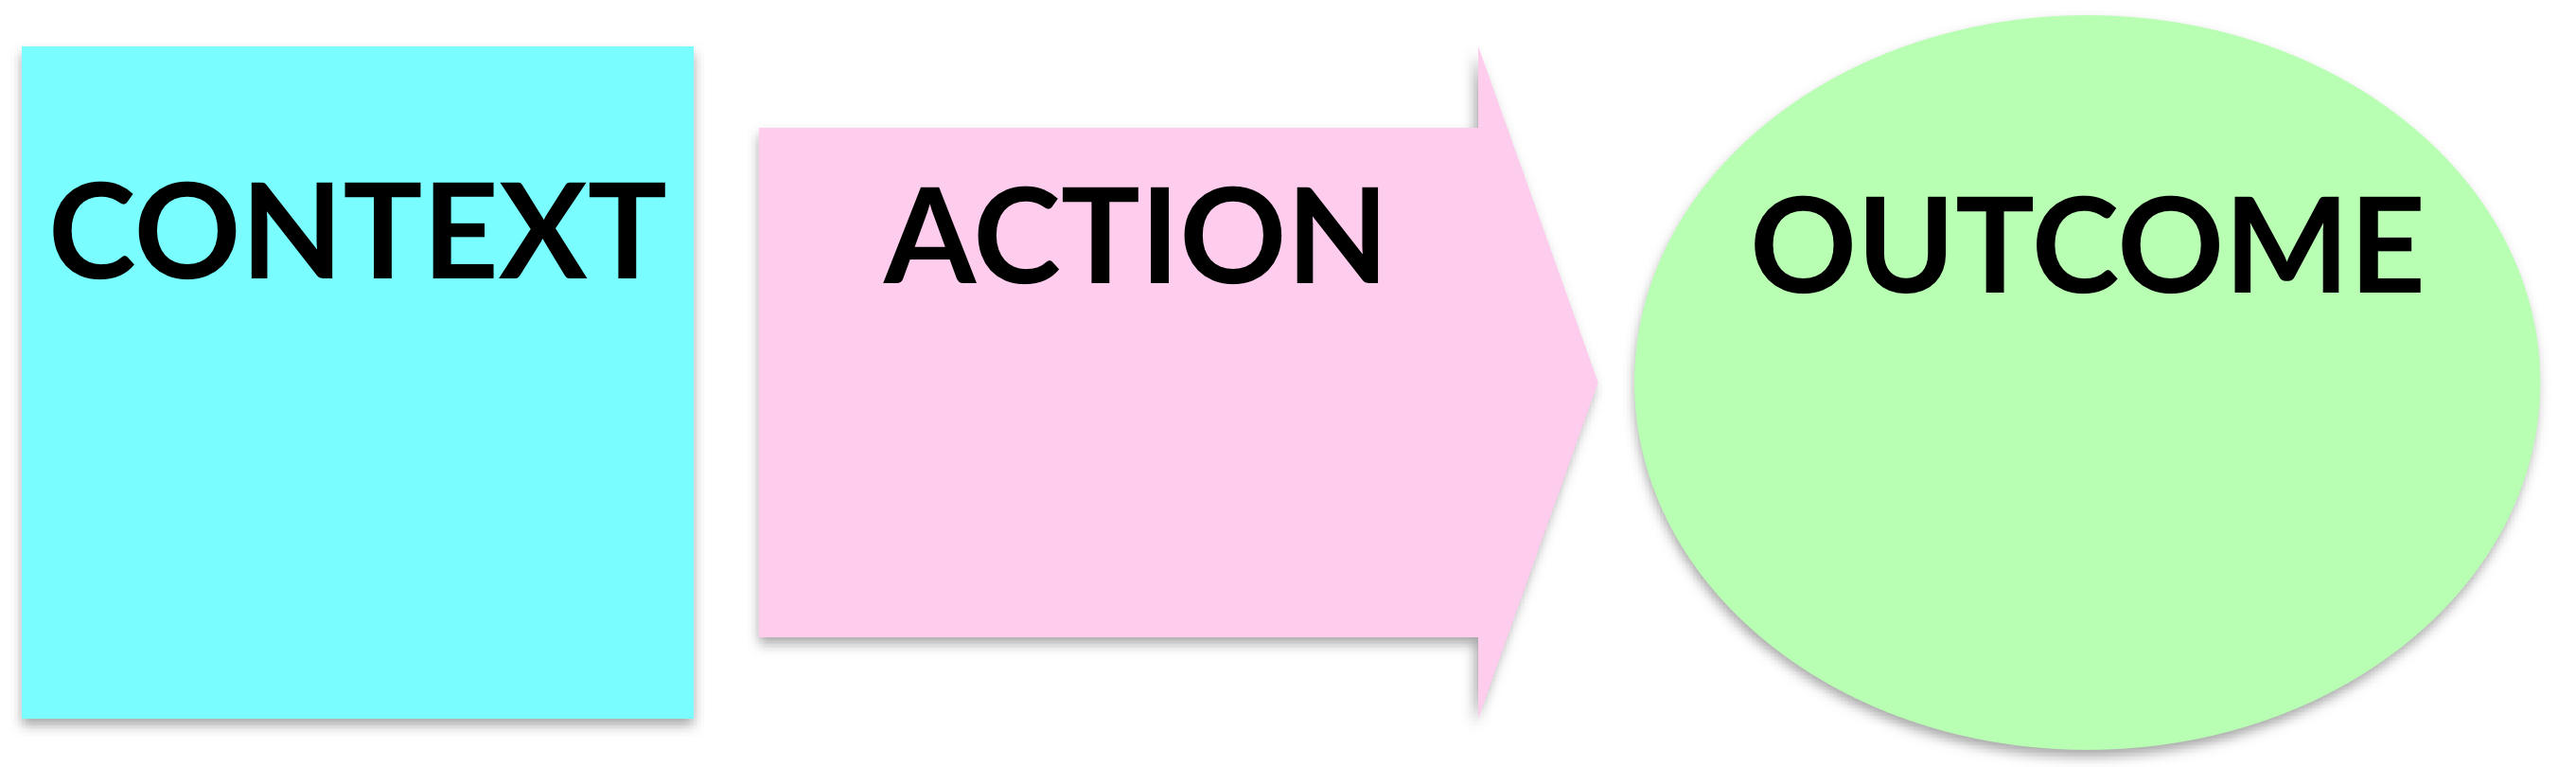
\includegraphics[width=\textwidth, keepaspectratio]{images/context-action-outcome}
\end{center}

\QandAbox{Look back at the examples you wrote during the library exercise. Do any of them omit any of these three parts?}{3}

\QandAbox{What level of detail should be included in an example?}{3}

\QandAbox{Can you think of an example that includes the words \emph{three minutes later} in the \emph{action}?}{3}